\cleardoublepage
\chapter{Related Work}
\label{ch:relatedwork}
\label{ch:chapter2}

\section{Referential Framework}

In this section, we introduce the relevant concepts used throughout this work. We cover foundational theory including Large Language Models, Retrieval Augmented Generation, as well as, advanced topics such as a formal introduction of language agents.

\subsection{Long-Context LLMs}

Various mechanisms have long been studied in Natural Language Processing for modeling long-term dependencies. Before the introduction of the transformer architecture, Recurrent Neural Networks (RNNs) represented the state of the art. RNNs maintain a hidden state that recursively propagates through the sequence, allowing them to encode information from previous tokens as context for later inputs \cite{alma991005389998907681}. However, RNNs were both prohibitively expensive to train and difficult to optimize due to issues like vanishing and exploding gradients \cite{dai-etal-2019-transformer}.

\noindent Transformer-based architectures addressed many of these challenges by replacing recurrence with a self-attention mechanism, which enables each token to attend to all others in the input sequence \cite{10.5555/3295222.3295349}. This design has facilitated a wide range of applications, such as conversational agents. However, the self-attention block incurs a time and space complexity of $O(n^2)$ with respect to the sequence length $n$, making it costly to extend context windows with this approach alone \cite{pmlr-v201-duman-keles23a}\cite{wang2023augmentinglanguagemodelslongterm}. 

\noindent To mitigate these limitations, some recent architectures have attempted to introduce recurrence into transformers, though such methods often suffer from information loss over long sequences \cite{dai-etal-2019-transformer}. Other strategies, such as positional interpolation, rescale position indices to align with those used during pretraining. While effective in some cases, these methods are limited to RoPE-based LLMs, and certain configurations, such as static YARN,  have been shown to significantly degrade performance on shorter texts \cite{ding2024longrope}\cite{peng2024yarn}.
Another line of work explores external memory modules or residual side networks that persist information across inputs \cite{wang2023augmentinglanguagemodelslongterm}. However, these remain constrained by architecture-specific limitations.

\noindent Overall, while this area of research is promising, it represents significant challenges. Embedding all information directly into the context window increases token usage and computational cost. Moreover, as more content is added, it becomes increasingly difficult for the model to effectively attend to the most relevant information, often resulting in reduced performance \cite{liu2023lostmiddlelanguagemodels}\cite{leng2024longcontextragperformance}.

\subsection{Retrieval Augmented Generation}
\label{subsec:rag}

Retrieval Augmented Generation enhances LLMs by integrating relevant knowledge from external sources into their context. Rather than relying solely on parametric memory, RAG retrieves supporting facts from external knowledge sources, making it a cost-effective and widely adopted approach for providing accurate and up-to-date information to the model \cite{lewis2021retrievalaugmentedgenerationknowledgeintensivenlp}. Figure \ref{fig:rag} illustrates a standard RAG pipeline for a QA task.

\begin{figure}[h]
    \centering
    \includegraphics[width=0.95\textwidth]{images/rag.pdf}\\[-0.25cm]
    \caption{A typical RAG pipeline for a QA task. A retriever selects relevant documents from an external source based on the input question. The retrieved context is then passed to an LLM, which generates the final answer \cite{yaosu2024racm3}.}
    \label{fig:rag}
\end{figure}

\noindent Researchers have explored different retrieval granularities, including document chunks, summaries, and knowledge triples \cite{zeng2024structuralmemoryllmagents}, as well as diverse retrieval algorithms such as sparse methods (e.g., BM25) and dense embeddings. Dense vector embeddings, in particular, have become widely adopted. They encode text semantics into fixed-dimensional representations, typically ranging from a few hundred to several thousand dimensions. However, single-vector representations face fundamental limitations, they cannot effectively capture all possible top-$k$ combinations of relevant documents for a given query \cite{weller2025theoreticallimitationsembeddingbasedretrieval}. To address this, researchers have developed multi-vector embeddings, where documents are represented using multiple vectors instead of one. This richer representation has been shown to outperform single-vector methods in many scenarios \cite{santhanam-etal-2022-colbertv2}.

\noindent More advanced RAG architectures involve additional components. For example, some systems use a second-stage retriever to re-rank the initial retrieval set. Sun et al. investigated whether LLMs can be trained as re-rankers, concluding that they indeed outperform state-of-the-art supervised methods \cite{sun-etal-2023-chatgpt}.

\noindent Graph RAG, an alternative RAG architecture, uses an LLM to extract entities and relationships from a corpus to construct a knowledge graph, which enables more effective reasoning over structured data, a strategy particularly useful for answering global questions where conventional RAG methods often underperform  \cite{edge2024localglobalgraphrag}. HippoRAG, inspired by neurobiological systems, also adopts a graph-based design and has shown promising results \cite{NEURIPS2024_6ddc001d}.

\noindent Unfortunately, RAG alone has been proven insufficient for tasks requiring complex reasoning, such as MHQA. Scaling RAG often leads to diminishing returns, with performance plateauing beyond a certain point \cite{leng2024longcontextragperformance}. This suggests that retrieval must be complemented by more sophisticated reasoning capabilities to effectively handle the complexity and volume of information in QA tasks.

\subsection{Prompt Engineering}

Numerous prompting methods have been developed to enhance the capabilities of LLMs, enabling them to reason over complex datasets. Techniques such as \textbf{Few-Shot Prompting} and \textbf{Chain of thought (CoT)} have shown impressive results in tasks such as mathematical reasoning \cite{wei2023chainofthoughtpromptingelicitsreasoning}. Few-Show Prompting consists of providing the model with input-output examples that serve as guidance, a process often referred to as \textit{in-context learning}. CoT, on the other hand, strengthens reasoning by generating intermediate reasoning steps before producing a final answer. These two methods can also be combined, as illustrated in Figure \ref{fig:few-shot-prompt}.

\begin{figure}[h]
    \centering
    \lstinputlisting{./chapter2/few-shot-prompt.txt}
    \caption{Example of a one-shot prompt combined with CoT to solve a multi-step mathematical problem.}
    \label{fig:few-shot-prompt}
\end{figure}

\noindent Other prompting methods directly integrate reasoning and interaction. For example, \textbf{ReAct} generates both reasoning traces and textual actions in an interleaved manner. This framework allows models to interact with external environments, gather observations, and update their reasoning in a cycle \cite{yao2023react}\cite{language-agent-tutorial}.

\begin{figure}[h]
    \centering
    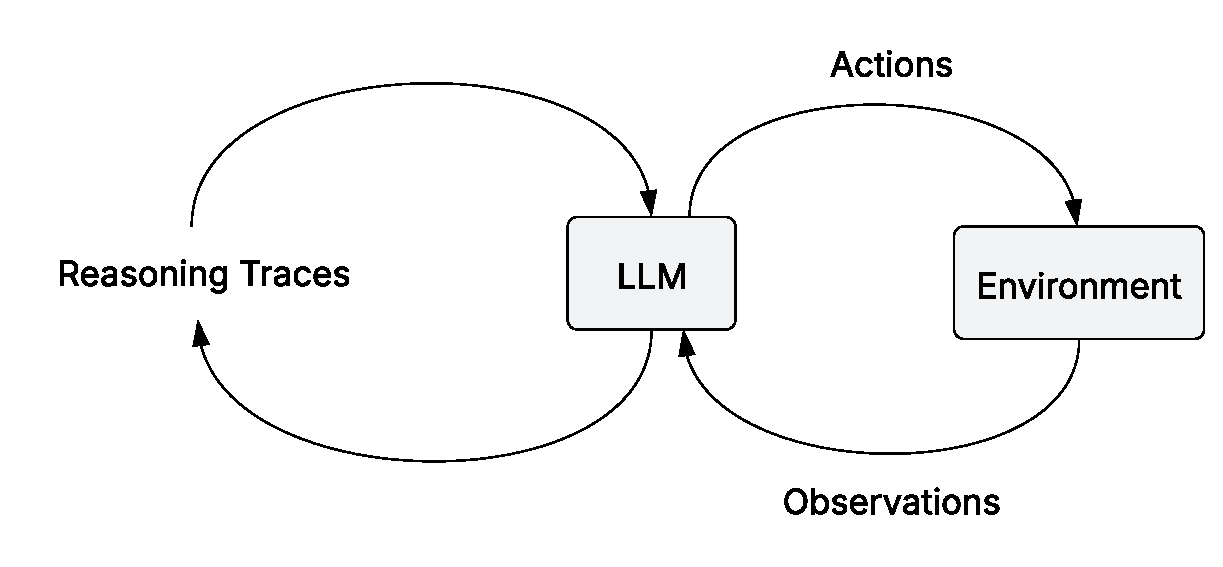
\includegraphics[width=0.95\textwidth]{images/react}\\[-0.25cm]
    \caption{The ReAct framework, which interleaves reasoning and action, enabling models to interact with the environment while maintaining reasoning traces \cite{yao2023react}.}
    \label{fig:react}
\end{figure}

\noindent For long documents, \textit{\textbf{PEARL}} (\textbf{P}lanning with \textbf{E}xecutable Actions for \textbf{R}easoning over \textbf{L}ong documents) introduces a three-stage prompting strategy. First, an LLM generates a list of text-based actions that could support answering a question. For example, an action might be ANALYZE(X, Y, CTX), which examines the relationship between entities X and Y within a given context CTX. Second, Given a question, the LLM produces a step-by-step plan using the previously generated actions. Finally, the LLM executes the plan on the full document, applying each action in order to generate the final answer. This framework is specifically designed to enhance comprehension and reasoning when operating over long contexts \cite{sun-etal-2024-pearl}. 

\noindent Similarly, \textit{\textbf{Iterative Demonstration-Based RAG}}, proposed by Yue et al, addresses complex queries by decomposing them into simpler sub-queries. RAG is then applied to each sub-query independently, leading to improved performance over single-pass RAG methods \cite{yue2024inferencescalinglongcontextretrieval}.

\noindent Further exploration of how various prompting methods can be integrated with language agents remains a fascinating area of research \cite{trivedi-etal-2023-interleaving}. Understanding how these methods scale and interact with different RAG strategies is crucial for advancing the capabilities of language agents in handling complex reasoning and planning \cite{language-agent-tutorial}.

\subsection{Language Agents}

An agent is broadly defined as a system that can perceive its environment, reason about it, and autonomously take actions to achieve specific goals. Traditional agents have relied on symbolic reasoning or domain-specific heuristics, but recent advances in LLMs have enabled a new class of agents.

\noindent Language Agents are autonomous systems that integrate LLMs for reasoning and communication, using language as their primary medium of interaction with both the environment and decision-making processes \cite{language-agent-tutorial}. Figure \ref{fig:cognitive-arch} provides a high-level overview of the cognitive architecture behind these systems.

\noindent A central component of language agents is memory, which allows them to store and retrieve information. This capability supports learning from experience, maintain coherence over long interactions, and making more informed decisions. Drawing inspiration from human cognition, memory in language agents is often categorized into four types: \textit{episodic memory}, which stores past experiences; \textit{semantic memory}, which encodes factual knowledge; \textit{procedural memory}, which captures rules or functions; and \textit{working memory}, which manages short-term, task-relevant information \cite{sumers2024cognitive}.

\noindent Several systems embody these concepts in different ways. MemGPT, for example, manages multiple storage tiers and leverages episodic and semantic memory for retrieval \cite{packer2024memgptllmsoperatingsystems}. While Graph Reader encodes knowledge in graph structures to support reasoning over long inputs \cite{li2024graphreaderbuildinggraphbasedagent}. AriGraph integrates episodic and semantic memories within a unified knowledge graph, enabling the agent to access structured information for more complex reasoning tasks \cite{anokhin2024arigraphlearningknowledgegraph}.

\begin{figure}[h]
    \centering
    \includegraphics[width=0.95\textwidth]{images/cognitive-arch.pdf}\\[-0.25cm]
    \caption{Cognitive architectures for language agents \cite{sumers2024cognitive}.}
    \label{fig:cognitive-arch}
\end{figure}

\noindent Language agents can also be augmented with external tools. The ability of LLMs to process structured formats such as JSON or XML facilitates integration with domain-specific APIs and databases \cite{language-agent-tutorial}. AriGraph, for instance, uses this capability to navigate a knowledge graph and retrieve relevant information for QA tasks \cite{anokhin2024arigraphlearningknowledgegraph}.

\noindent The reasoning and planning capabilities of language agents become particularly powerful when combined with prompting strategies designed to guide multi-step reasoning. ReAct \cite{yao2023react}, for instance, interleaves reasoning and action, helping agents analyze their environment, make decisions and execute plans.

\noindent Recent work has also explored multi-agent systems, where  agents collaborate or debate to solve a task \cite{language-agent-tutorial}. For example, Zhao et al. introduced a collaborative framework for QA over long documents in which a leader agent partitions a document into $m$ chunks, delegates each chunk to a worker agent, and aggregates their responses until a confident answer is reached \cite{zhao-etal-2024-longagent}.

\noindent Although language agents have been studied in diverse settings, including text-based games, human simulacra, and task automation \cite{10.1145/3586183.3606763}\cite{anokhin2024arigraphlearningknowledgegraph}, questions remain about their role in natural language tasks such as QA and MHQA. In particular, further exploration is needed to understand how planning and memory, when combined with techniques like RAG and prompt engineering, can contribute to more effective and adaptable systems in these domains.

\subsection{Question Answering}

Question Answering (QA) is a foundational task in natural language processing that involves predicting an answer given a question and some context. Recent advances in LLMs have led to significant progress in this area, enabling the development of systems that perform well across a range of diverse datasets and domains \cite{10.1561/1500000102}.


\noindent Despite these improvements, certain QA sub-tasks remain challenging. For instance, Textbook Question Answering (TQA) poses difficulties due to its reliance on long passages, as well as the integration of visual elements such as diagrams and tables \cite{ALAWWAD2025111332}.

\noindent Another challenging variant is Multi-Hop Question Answering (MHQA), where answering a question requires combining information from multiple sources or passages. Unlike single-hop QA, where a single context snippet typically contains the answer, MHQA requires reasoning over multiple facts or steps to arrive at a correct response \cite{10.1561/1500000102}. See Table \ref{tab:questions} for various examples of MHQA questions.

\input{chapter2/questions}

\subsection{Evaluation Metrics}

A variety of evaluation metrics have been established in the literature to assess QA systems, covering both retrieval quality and answer quality.

\subsubsection{Retrieval Metrics}

\noindent Let $Q$ denote the set of queries. For each query $q \in Q$, we define:

\begin{itemize}
    \item[] $R_q$: The number of relevant documents for query $q$
    \item[] $r_q$: The number of relevant documents retrieved for query $q$
    \item[] $k_q$: The total number of unique documents retrieved for query $q$
\end{itemize}

\noindent For unranked retrieval sets, macro-averaged metrics are commonly reported, ensuring equal weight is assigned to each query.

\begin{description}
    \item[Macro Retrieval (R)] The fraction of relevant documents returned by the system, averaged across queries \cite{Manning_Raghavan_Schütze_2008}:

    \begin{equation}
        \text{Macro Retrieval (R)} = \frac{1}{|Q|} \sum_{q \in Q} {\frac{r_q}{R_q}}
    \end{equation}
    \item[Macro Precision (P)] The fraction of retrieved documents that are relevant, averaged across queries \cite{Manning_Raghavan_Schütze_2008}:

    \begin{equation}
        \text{Macro Precision (P)} = \frac{1}{|Q|} \sum_{q \in Q} {\frac{r_q}{k_q}}
    \end{equation}

    \item[Macro $F_1$] The $F_1$ score for each query is the harmonic mean of its precision and recall. Macro $F_1$ is the average of these query-level $F_1$ scores \cite{Manning_Raghavan_Schütze_2008}:

    \begin{equation}
        \text{Macro $F_1$} = \frac{1}{|Q|} \sum_{q \in Q} {F_1(q)}
    \end{equation}
\end{description}

\noindent For ranked retrieval sets, \textbf{retrieval@K} \cite{Manning_Raghavan_Schütze_2008} is commonly used. Let $r_q@K$ be the number of relevant documents retrieved within the top-$k$ documents for query $q$. Then:

\begin{equation}
    \label{eq:mrk}
    \text{Macro retrieval@K} = \frac{1}{|Q|} \sum_{q \in Q} {\frac{r_q@K}{R_q}}
\end{equation}

\subsubsection{Question Answering Metrics}

\noindent For QA evaluation, different metrics are commonly employed to evaluate answer quality.

\begin{description}
    \item[Exact Match (EM)] is the strictest measure, assigning a score of 1 only when the predicted answer exactly matches the reference. While simple and widely used in QA benchmarks, EM often penalizes semantically correct answers that differ in form (e.g., synonyms, paraphrases, or even formatting differences) \cite{tang-etal-2021-multi}.
    \item[ROUGE] originally developed for text summarization and translation, compares the overlap of n-grams between prediction and reference answers. Among its many variants, ROUGE-1 ($R_1$) and ROUGE-2 ($R_2$) are the most common, evaluating unigram and bigram overlaps, respectively \cite{lin-2004-rouge}. $R_1$ is equivalent to an $F_1$ score, with a small constant $\epsilon=1 \times 10^{-8}$ added to avoid division by zero \cite{mrqa-2021-machine}. Despite its ability to capture partial matches, ROUGE still overlooks semantic equivalence when answers differ in wording.
    \par
    \begin{equation}
        \text{ROUGE} = 2 \cdot \frac{\text{Precision} \cdot \text{Recall}}{\text{Precision} + \text{Recall} + \epsilon}
    \end{equation}
    \item[LLM Judge ($L_1$)] Human evaluation is a reliable method for assessing the quality of LLM-generated responses. However, it is both costly and time-consuming. Recently, LLM-based evaluators have gained popularity as a scalable alternative due to their ability to align well with human preferences \cite{zheng2023judgingllmasajudgemtbenchchatbot}. Their increasing adoption reflects their ability to approximate human judgment at scale. LLM judges can be used as a binary evaluator \cite{li2024llmsasjudgescomprehensivesurveyllmbased}, which assigns a score of 1 if it determines that the predicted and reference answers are semantically equivalent. Formally:

    \begin{equation}
        \text{$L_1$} = \frac{1}{|Q|} \sum_{q \in Q} {j_q}
    \end{equation}

    where $j_q = 1$ if the LLM judge considers the answer correct, and $j_q = 0$ otherwise.
\end{description}

\noindent While other evaluation metrics such as BERTScore exist, this measure is not always well-suited for QA scenarios. BERTScore computes similarity between reference and predicted answers by comparing token embeddings from a pretrained language model \cite{zhang2020bertscoreevaluatingtextgeneration}, making it effective for capturing semantic similarity. However, in entity-centric datasets, BERTScore may assign high scores to incorrect answers when entities are close in the embedding space but are, in fact, completely different entities.

\noindent In our work, we place particular emphasis on $R_1$ and $L_1$, as they provide more flexibility in recognizing semantically correct answers. Our decision is consistent with prior work \cite{chen-etal-2019-evaluating}, and these metrics are well-suited for evaluating both retrieval and answer generation in the QA and MHQA tasks.

\section{State of the art}

This section reviews state-of-the-art (SOTA) approaches for both QA and MHQA, outlining their core concepts and possible limitations.

\subsection{HippoRAG}

HippoRAG, briefly introduced in Section \ref{subsec:rag}, is a RAG system that achieves SOTA performance on several QA benchmarks. The framework operates in two phases: offline indexing and online retrieval.

\noindent In the offline phase, an instruction-tuned LLM is prompted to extract named entities from the corpus. These entities serve as input for a second prompt based on OpenIE, which produces knowledge triples \cite{NEURIPS2024_6ddc001d}. For example, given the passage.

\begin{quote}
    Nicholas J. Belkin is a professor at the School of Communication and Information at Rutgers University. Among the main themes of his research are digital libraries; information-seeking behaviors; and interaction between humans and information retrieval systems.
\end{quote}

\noindent The system identifies entities such as \textit{Nicholas J. Belkin}, \textit{School of Communication and Information at Rutgers University}, and \textit{digital libraries}. It then generates triples like (\textit{Nicholas J. Belkin}, \textit{is}, \textit{Professor}), and (\textit{Nicholas J. Belkin}, \textit{researches}, \textit{digital libraries}). These triples form a graph of entities and relations. To enrich the graph, HippoRAG uses a dense embedding model to detect semantically similar entities above a similarity threshold, adding additional edges \cite{NEURIPS2024_6ddc001d}.

\noindent In the online retrieval phase, an LLM extracts named entities from the query. These entities are encoded using the embedding model and matched to graph nodes via cosine similarity. The top-matched nodes are selected as query nodes and serve as seeds for a Personalized Page Rank algorithm (PPA). PPR propagates probability mass through the graph starting from these query nodes, assigning high scores to nodes in their local neighborhoods. The resulting ranking scores determine the final retrieval set \cite{NEURIPS2024_6ddc001d}.

\begin{figure}[h]
    \centering
    \includegraphics[width=0.95\textwidth]{images/hipporag.png}\\[-0.25cm]
    \caption{HippoRAG architecture: (i) Offline indexing, where an LLM extracts entities and relations to construct a graph, and (ii) online retrieval, where entities from the query guide context-based retrieval \cite{NEURIPS2024_6ddc001d}.}
    \label{fig:hippo_rag}
\end{figure}

\noindent Rather than relying on multi-step retrieval, HippoRAG retrieves all relevant passages in a single pass. Authors show that it outperforms alternatives such as ColBERTv2, particularly on challenging datasets like MuSiQue and 2Wiki \cite{trivedi2021musique, ho-etal-2020-constructing}. Moreover, HippoRAG is complementary to other SOTA methods, such as IRCoT, which uses iterative retrieval \cite{trivedi-etal-2023-interleaving}.

\noindent Their evaluation is based on a relatively small sample of 1,000 questions per dataset, making comparisons to other approaches difficult. More recent extensions propose incorporating both conceptual and contextual information into the graph and filtering triples to retain only the most relevant nodes during online retrieval \cite{gutiérrez2025ragmemorynonparametriccontinual}.

\noindent In this work, we explore how cognitive language agents compare against such RAG frameworks, and further explore how they can be integrated into agentic workflows.

\subsection{PAR RAG}

PAR RAG is a RAG framework designed for MHQA tasks. It is composed of three modules: planning, acting, and review.

\noindent The planning module generates a top-down plan that decomposes the original question into sub-questions using an LLM. 

\noindent The action module executes the plan step by step using ColBERTv2 as the retriever. At each step, a preliminary answer is generated, which is then passed to the review stage.

\noindent The review module verifies the credibility of the intermediate answer, correcting potential mistakes to prevent error propagation. To support this process, an additional retrieval step using the preliminary answer is triggered, providing relevant evidence that strengthens the review and validation.

\begin{figure}[h]
    \centering
    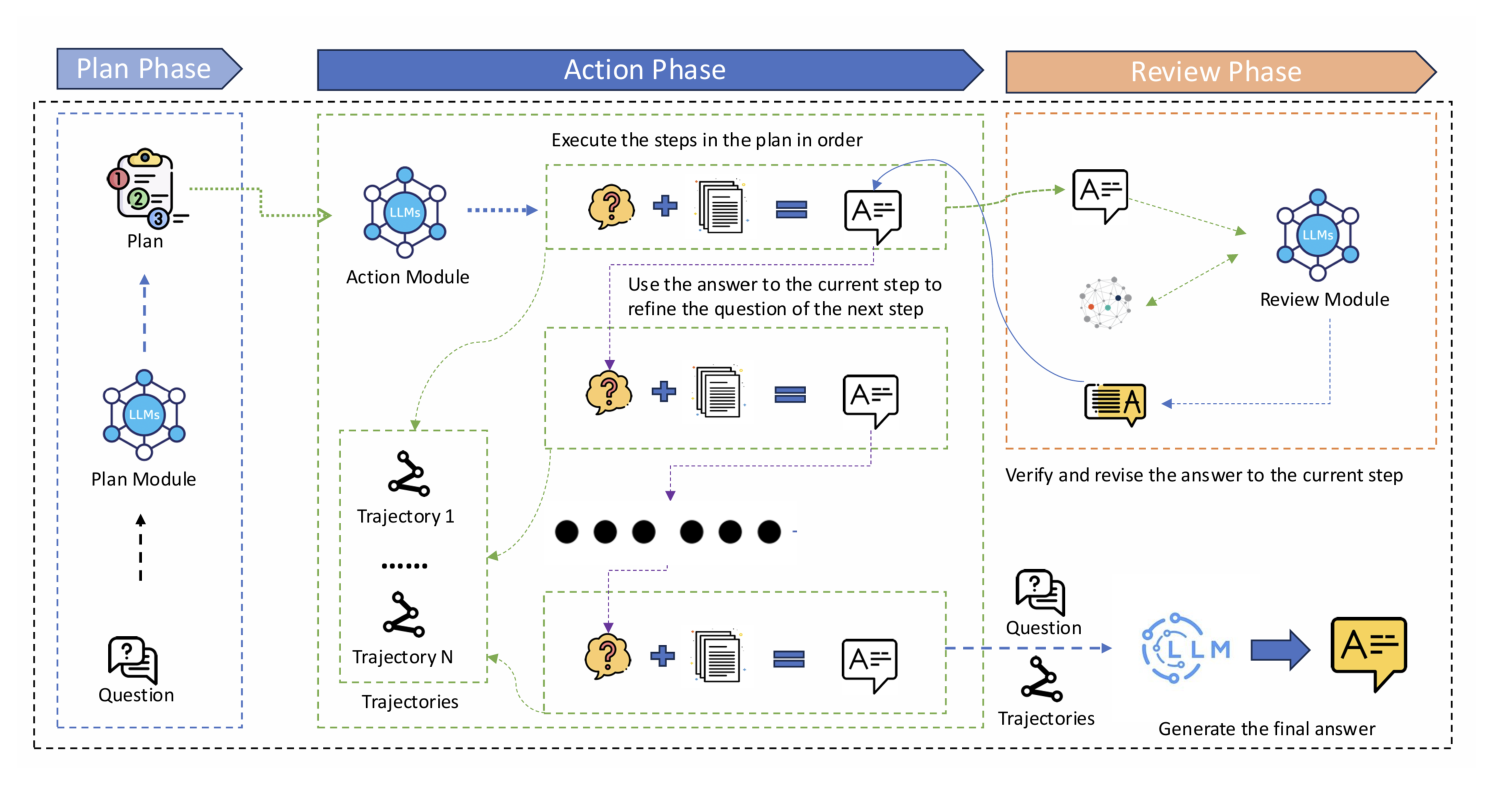
\includegraphics[width=0.95\textwidth]{images/par_rag.eps}\\[-0.25cm]
    \caption{PAR RAG framework: (i) Plan Phase, where an LLM decomposes the question into a structured sequences of sub-questions, (ii) Action Phase, where the plan is executed step by step, and intermediate results are produced, and (iii) Review Phase, where each intermediate answer is validated with an LLM to prevent error propagation \cite{zhang2025credibleplandrivenragmethod}.}
    \label{fig:par_rag}
\end{figure}

\noindent This design makes the system more robust against reasoning or retrieval errors, as intermediate mistakes are less likely to cascade through the full reasoning chain. Once all sub-questions have been answered and verified, an LLM synthesizes the original question together with the intermediate results to generate the final answer.

\noindent Empirical results show that PAR RAG outperforms previous RAG methods on challenging MHQA benchmarks. For example, it achieves nearly a 12-point improvement in $F_1$ score on MuSiQue compared to HippoRAG.

\noindent In our work, we adopt similar architectural principles, but we frame them under the broader concept of cognitive language agents.
